\documentclass[letterpaper,12pt,fleqn]{article}
\usepackage{matharticle}
\usepackage{tikz}
\pagestyle{plain}
\renewcommand{\P}{\mathcal{P}}
\begin{document}

\begin{center}
  \large
  Math-42 Sections 01, 02, 05

  \Large
  Homework \#8 Solutions
\end{center}

\subsection*{Problems}

Consider \(f:A\to B\) and let \(S,T\subseteq A\).

\begin{enumerate}[left=0in]
\item Prove: \(f(S\cap T)\subseteq f(S)\cap f(T)\)

  \bigskip

  Assume \(y\in f(S\cap T)\) \\
  \(\exists\,x\in S\cap T,y=f(x)\) \\
  \colorbox{red!25!white}{\(x\in S,y=f(x)\) and \(x\in T,y=f(x)\)} \\
  \colorbox{red!25!white}{\(y\in f(S)\) and \(y\in f(T)\)} \\
  \(y\in f(S)\cap f(T)\) \\
  \(\therefore f(S\cap T)\subseteq f(S)\cap f(T)\)

  \bigskip
  
\item Draw a diagram that shows why this is a subset relationship and not set equality.  In other words, show why
  there can be elements in \(f(S)\cap f(T)\) that are not in \(f(S\cap T)\).

  \bigskip

  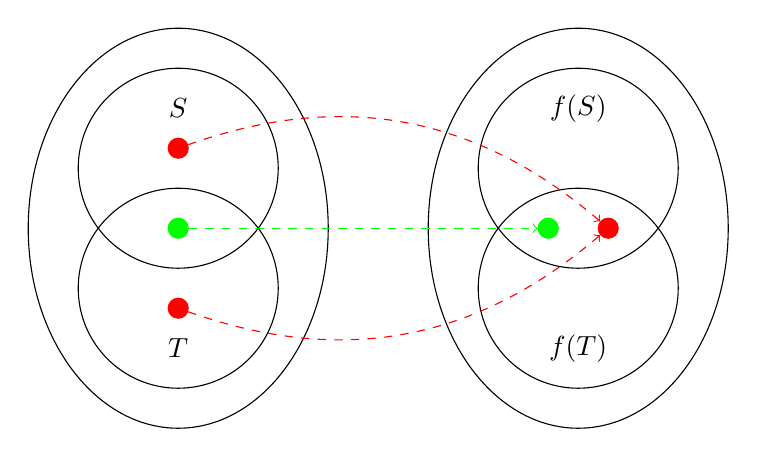
\begin{tikzpicture}
    \draw (0,0) ellipse (0.75in and 1in);
    \draw (0,0.3in) circle [radius=0.5in];
    \node at (0,0.6in) {\(S\)};
    \draw (0,-0.3in) circle [radius=0.5in];
    \node at (0,-0.6in) {\(T\)};
    \draw (2in,0) ellipse (0.75in and 1in);
    \draw (2in,0.3in) circle [radius=0.5in];
    \node at (2in,0.6in) {\(f(S)\)};
    \draw (2in,-0.3in) circle [radius=0.5in];
    \node at (2in,-0.6in) {\(f(T)\)};
    \node (X) [draw,circle,fill,color=green,inner sep=0in,minimum size=0.1in] at (0,0) {};
    \node (Y1) [draw,circle,fill,color=green,inner sep=0in,minimum size=0.1in] at (1.85in,0) {};
    \draw [->,dashed,green] (X) -- (Y1);
    \node (X1) [draw,circle,fill,color=red,inner sep=0in,minimum size=0.1in] at (0,0.4in) {};
    \node (X2) [draw,circle,fill,color=red,inner sep=0in,minimum size=0.1in] at (0,-0.4in) {};
    \node (Y2) [draw,circle,fill,color=red,inner sep=0in,minimum size=0.1in] at (2.15in,0) {};
    \draw [->,dashed,red] (X1) edge [bend left] (Y2);
    \draw [->,dashed,red] (X2) edge [bend right] (Y2);
  \end{tikzpicture}

  \bigskip

\item How can \(f\) be limited so that equality occurs.  In other words, how do you eliminate the problem in
  your drawing?

  \bigskip

  Require that \(f\) be injective.  Thus, the problem case in the diagram does not occur.

  \bigskip
  
\item Which step in your proof is not reversible?

  \bigskip

  The transition shown in red is the problem.  Going in the forward direction, we are talking about the same \(x\).
  Going in the reverse direction, there could be two separate \(x\) values.
\end{enumerate}

\end{document}
